\documentclass[11pt]{article}
\usepackage[margin=1in]{geometry}
\usepackage{amsmath,amssymb,amsthm}
\usepackage{graphicx}
\usepackage[hidelinks]{hyperref}

\newtheorem{theorem}{Theorem}
\newtheorem{lemma}{Lemma}

\newcommand{\cS}{\mathbb S}
\newcommand{\ccard}{\mathfrak c}
\newcommand{\omegaone}{\omega_1}
\newcommand{\iso}{\simeq}
\newcommand{\notiso}{\not\simeq}
\newcommand{\Sz}{\operatorname{Sz}}

\title{A Negative Answer to the Double Arrow Ordinal Product Question}
\author{Run \texttt{fa\_banach\_001}, lane 14}
\date{2026-06-29}

\begin{document}
\maketitle

\noindent\textbf{Status.} \texttt{full\_solution\_likely\_valid}.

\section{Source Question and Criterion}

The source paper is Korpalski, \emph{Semadeni-Pelczynski derivative and
Banach spaces of continuous functions on nonmetrizable cubes},
arXiv:2502.16981 \cite{Korpalski}. Let $\cS$ denote the double arrow space.
Question 1 on page 22 asks whether
\[
  C(\cS) \iso C(\cS\times [0,\alpha])
\]
for every ordinal $\omega^\omega\leq \alpha<\omega_1$.

Immediately after the question, Proposition 6.2 of the same source gives the
following obstruction:
if $K$ is compact and $C(K)$ does not embed into $c_0(\ccard)$, then
\[
  C(\cS)\notiso C(\cS\times K).
\]

\begin{center}
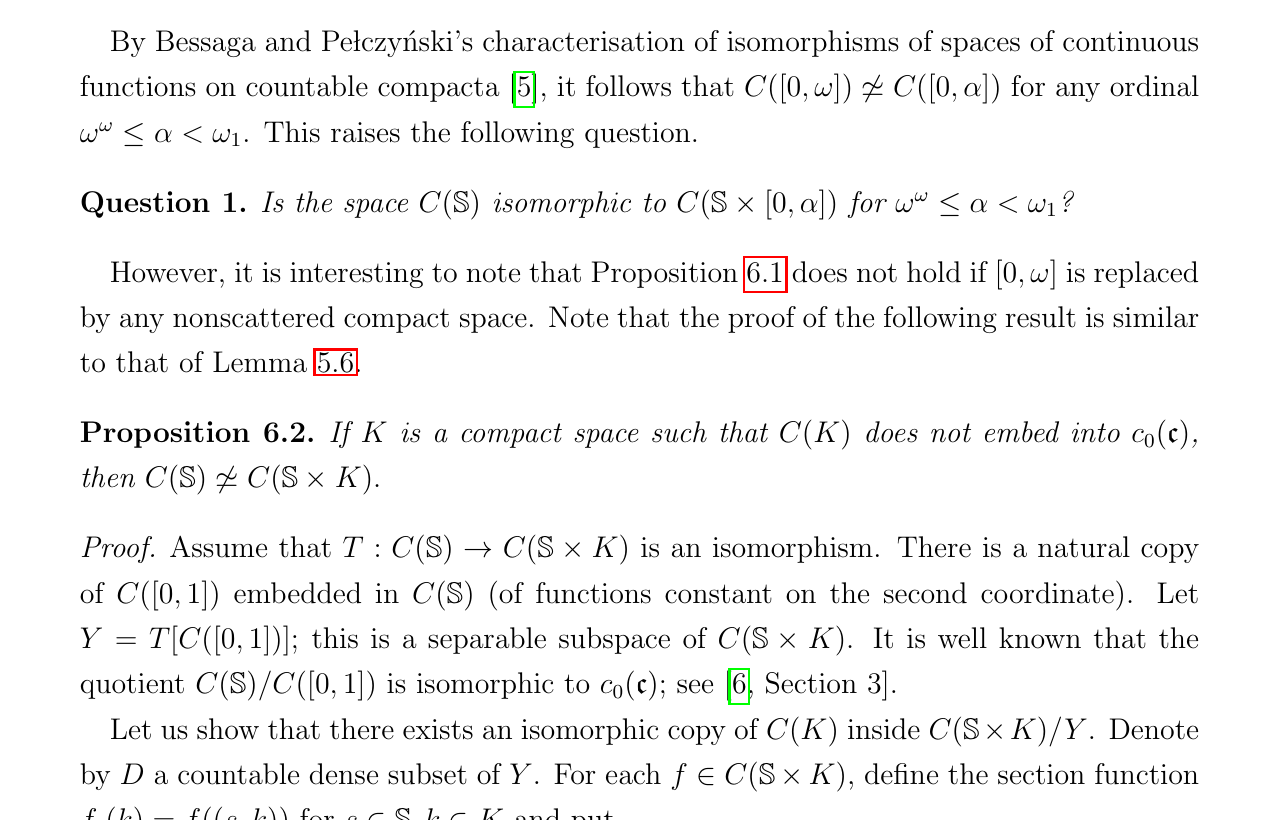
\includegraphics[width=0.97\linewidth]{figures/question_and_criterion_crop.png}
\end{center}

\section{Key Observation}

For $K=[0,\alpha]$ with $\omega^\omega\leq\alpha<\omega_1$, the space
$C(K)$ is separable but has Szlenk index strictly larger than that of $c_0$.
Consequently $C(K)$ cannot embed into $c_0(\ccard)$.

The separability point is useful because every separable subspace of
$c_0(\ccard)$ is contained in $c_0(A)$ for some countable
$A\subseteq\ccard$, hence in a copy of ordinary $c_0$. The Szlenk obstruction
then applies in the separable space $c_0$.

\section{Non-Embedding Lemma}

\begin{lemma}\label{lem:nonembed}
Let $\omega^\omega\leq\alpha<\omega_1$. Then
$C([0,\alpha])$ does not embed isomorphically into $c_0(\ccard)$.
\end{lemma}

\begin{proof}
Suppose that $J:C([0,\alpha])\to c_0(\ccard)$ is an isomorphic embedding.
The range $J[C([0,\alpha])]$ is separable. Choose a countable dense set
$D$ in this range. For $y\in c_0(\ccard)$, the support
\[
  \operatorname{supp}(y)=\{\gamma<\ccard:y(\gamma)\neq 0\}
\]
is countable. Hence
\[
  A=\bigcup_{y\in D}\operatorname{supp}(y)
\]
is countable. Every coordinate outside $A$ vanishes on $D$, hence vanishes on
the closed range $J[C([0,\alpha])]$. Thus the range is contained in
$c_0(A)\iso c_0$.

By monotonicity of the Szlenk index under subspaces, this would give
\[
  \Sz(C([0,\alpha]))\leq \Sz(c_0)=\omega.
\]
But Brooker's computation of the Szlenk indices of ordinal intervals says that
if $\gamma$ is the unique ordinal satisfying
\[
  \omega^{\omega^\gamma}\leq\alpha<\omega^{\omega^{\gamma+1}},
\]
then
\[
  \Sz(C([0,\alpha]))=\omega^{\gamma+1}.
\]
For $\alpha\geq\omega^\omega$ one has $\gamma\geq 1$, so this index is at
least $\omega^2$, a contradiction.
\end{proof}

\section{Answer to Question 1}

\begin{theorem}
Let $\cS$ be the double arrow space. For every ordinal
$\omega^\omega\leq\alpha<\omega_1$,
\[
  C(\cS)\notiso C(\cS\times[0,\alpha]).
\]
Thus Question 1 of \cite{Korpalski} has a negative answer throughout the
range in which it is asked.
\end{theorem}

\begin{proof}
Fix $\omega^\omega\leq\alpha<\omega_1$ and put $K=[0,\alpha]$.
By Lemma \ref{lem:nonembed}, $C(K)$ does not embed into $c_0(\ccard)$.
Proposition 6.2 of the source paper therefore applies and gives
\[
  C(\cS)\notiso C(\cS\times K)
  =
  C(\cS\times[0,\alpha]).
\]
\end{proof}

\section{Verification Notes}

The proof uses two external inputs. The first is Proposition 6.2 of the source
paper. The second is the standard Szlenk-index computation for
$C([0,\alpha])$ due to Brooker \cite{Brooker}. The reduction from
$c_0(\ccard)$ to $c_0$ is included above: separable subspaces of
$c_0(\ccard)$ have countable coordinate support.

The run indexes were searched for the arXiv id, the double-arrow keywords, the
product question, $c_0(\ccard)$, Szlenk, and ordinal variants. Local source
searches found no prior packet for this exact consequence. Web searches on
2026-06-29 found Brooker's Szlenk computation and no separate exact resolution
of the double-arrow question.

\section{Limitations and Review Recommendation}

This is a counterexample-style resolution, not an independent reproving of
Proposition 6.2. Human review should check that the target protocol permits
using a later proposition from the source paper together with the classical
Szlenk computation. Mathematically, the main points to verify are the
countable-coordinate reduction inside $c_0(\ccard)$ and the cited Szlenk
formula for $\alpha\geq\omega^\omega$.

\begin{thebibliography}{9}
\bibitem{Korpalski}
M. Korpalski,
\emph{Semadeni-Pelczynski derivative and Banach spaces of continuous functions
on nonmetrizable cubes},
arXiv:2502.16981, 2025.

\bibitem{Brooker}
P. A. H. Brooker,
\emph{Szlenk and $w^\ast$-dentability indices of ordinal $C(K)$ spaces},
arXiv:1210.3696, 2012.
\end{thebibliography}

\end{document}
